\subsection{Analýza aplikačného rámca pre IPFIX Mediátor} \label{sec:framework}

Analýze aplikačného rámca pre sprostredkovanie správ v IPFIX sa venuje RFC 6183 \citep{rfc6183}. 
V nasledujucich kapitolách si podrobnejšie priblížime referenčný model a vybrané komponenty, či procesy 
aplikačného rámca.

\subsubsection{Referenčný model sprostredkovania správ v IPFIX}


Obrázok \ref{o:mediation_reference_model} predstavuje referenčný model sprostredkovania správ v IPFIX 
ako rozšírenie referenčného modelu IPFIX, popísaného v \emph{Architecture for IP Flow Information Export} 
\citep{rfc5470}. Táto schéma zobrazuje možné scenáre, ktoré môžu existovať v meracej architektúre.
Funkčné komponenty v rámci každej entity sú ohraničené zátvorkami []. Mediátor môže prijímať 
záznamy o toku od iných mediátorov a exportérov a prúd záznamov z iných zdrojov.
Za iné zdroje sa považujú nástroje iných protokolov, ako napríklad NetFlow exportéry \citep{rfc3954}. 
Spracovane dáta vo forme záznamov o toku potom exportuje jednému alebo viacerým kolektorom a mediátorom.


Zjednodušený model komponentov IPFIX mediátora je zobrazený na Obrázku \ref{o:mediator_component_model}. 
Mediátor obsahuje jeden alebo viac sprostredkovateľských procesov, hierarchicky uložených 
medzi jedným alebo viacerými exportovacími a zhromažďovacími procesmi. Tento model sa týka 
najbežnejšieho prípadu, kedy mediátor prijíma dátové záznamy od exportéra, alebo iného mediátora.

\begin{figure}[ht!]
\centering
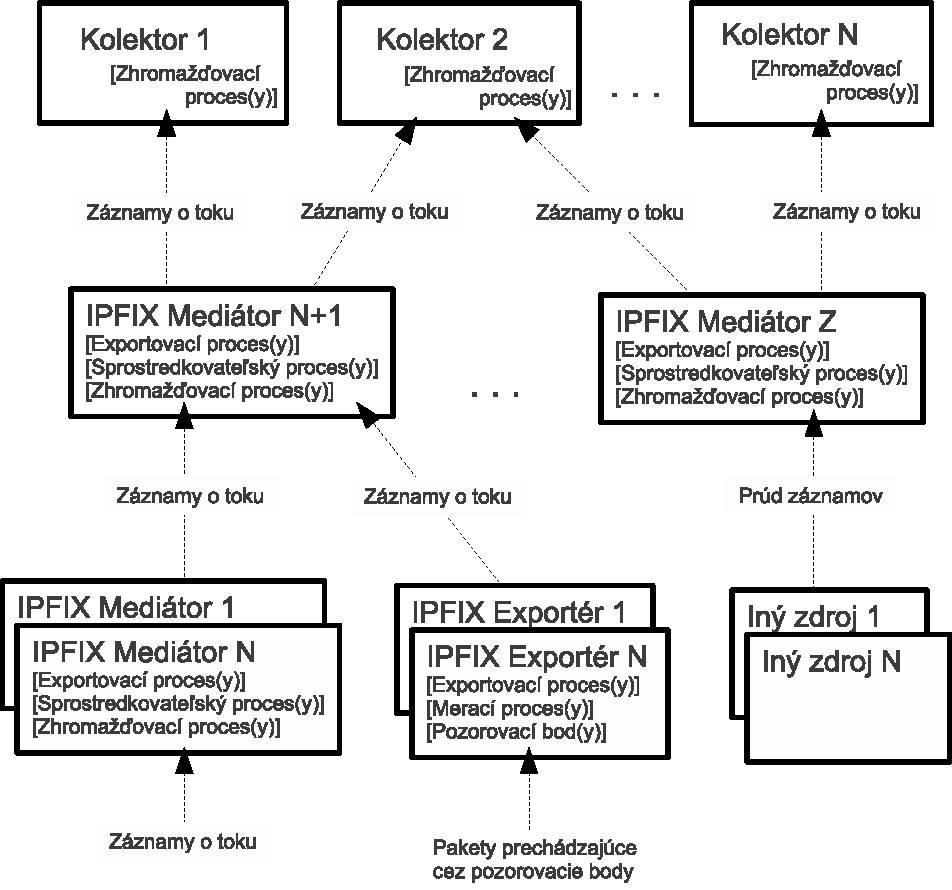
\includegraphics[width=0.9\textwidth]{mediation_reference_model}
\caption{Referenčný model sprostredkovania správ v IPFIX}\label{o:mediation_reference_model}
\end{figure}



\subsubsection{Komponenty sprostredkovania správ v IPFIX}

V nasledujúcich častiach si bližšie priblížime jednotlivé komponenty IPFIX mediátora, ktoré sú
znázornene na Obrázku \ref{o:mediator_component_model}.

\begin{figure}[ht!]
\centering
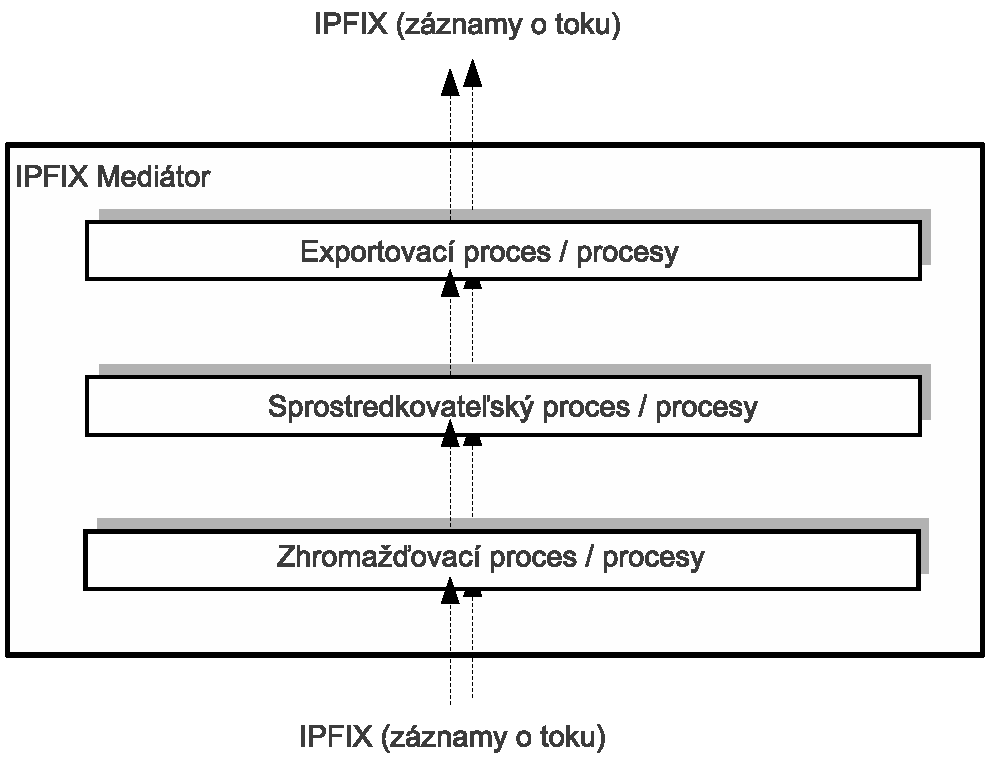
\includegraphics[width=0.7\textwidth]{mediator_component_model}
\caption{Zjednodušený model komponentov IPFIX Mediátora}\label{o:mediator_component_model}
\end{figure}


\paragraph{Zhromažďovací proces}

Zhromažďovací proces v IPFIX Mediátore sa nelíši od zhromažďovacieho procesu popísaného v 
špecifikácii IPFIX protokolu \citep{rfc5101}.
Jedinou funkciou naviac je odovzdanie sady dátových záznamov a riadiacich informácii jednému, alebo 
viacerým komponentom, tj. sprostredkovateľským procesom, alebo ďalším aplikáciam. 
To znamená, že zhromažďovací proces môže vytvárať kópie sady a prenášať ich buď sériovo, alebo paralelne.  
Medzi riadiace informácie patrí hlavička IPFIX správy, informácie o transportnej relácii, 
spolu s informáciami o meracom a exportovacom procese v exportéri, napr. vzorkovacie parametre.

\paragraph{Exportovací proces} \label{sec:exporting_process}

Exportovací proces IPFIX Mediátora sa vo svojej podstate tiež nelíši od toho, ktorý je popísaný v špecifikácii
protokolu \citep{rfc5101}.
Prídavné funkcie môžu byť nasledujúce:
\begin{itemize}
 \item Prijímať spúšťač \emph{trigger} od sprostredkovateľských procesov, ktorý vyvolá odoslanie správy
 kolektoru na odstránenie neplatnej šablóny \emph{(Template Withdrawal Message)}.
 \item Z dôvodu uvedeného v kapitole \ref{sec:loss_info} na strane \pageref{sec:loss_info}, je potrebné 
 preposielať informácie o pôvodcovi dát (exportérovi), napríklad ID pozorovacieho bodu a pozorovacej 
 domény, IP adresa exportéra atď. Exportovací proces tieto dáta zakóduje do prídavných dátových záznamov, 
 buď s využitím 
 informačných elementov skupiny 2 (tabuľka \ref{t:ie-group2}), alebo organizáciou špecifikovaných 
 elementov.
\end{itemize}

% ---- tabuľka ----
\tabcolsep=8pt
\begin{table}[!ht]\caption{Prehľad informačných elementov skupiny 2}\label{t:ie-group2}
\smallskip
\centering
\begin{tabular}{|c|c|}
\hline
\textbf{ID} & \textbf{názov informačného elementu} \\ \hline
130 & exporterIPv4Address \\ \hline
131 & exporterIPv6Address \\ \hline
217 & exporterTransportPort \\ \hline
211 & collectorIPv4Address \\ \hline
212 & collectorIPv6Address \\ \hline
213 & exportInterface \\ \hline
214 & exportProtocolVersion \\ \hline
215 & exportTransportProtocol \\ \hline
216 & collectorTransportPort \\ \hline
173 & flowKeyIndicator \\ \hline
\end{tabular}
\end{table}
% -----------

\paragraph{Sprostredkovateľské procesy} \label{sec:framework_intermediate}

Sprostredkovateľské procesy sú kľúčovými funkčnými blokmi sprostredkovania správ v IPFIX. Rôzne procesy 
pokrývajú každý príklad použitia sprostredkovania správ z kapitoly \ref{sec:mediator_examples} na strane 
\pageref{sec:mediator_examples}. 
Mediátor musí byť schopný súčasne podporovať viac ako jeden sprostredkovateľský proces. Spolupráca viacerých 
procesov je konfigurovaná nasledujúcimi spôsobmi.

\begin{itemize}
 \item \textbf{Paralelné spracovanie} - Prúd záznamov je spracovaný viacerými sprostredkovateľskými procesmi 
 paralelne tak, aby boli splnené požiadavky koncových aplikácií. V tomto scenári, každý 
 sprostredkovateľský proces dostáva kópiu celého prúdu záznamov ako vstup.
 \item \textbf{Sériové spracovanie} - Aby bolo zabezpečené flexibilné spracovanie prúdu záznamov, sprostredkovateľské
 procesy sú zapojene sériovo. V tomto prípade výstupný prúd záznamov jedného procesu je vstupným prúdom 
 nasledujúceho.
\end{itemize}






















